\documentclass[12pt]{beamer}
\usepackage{../Estilos/BeamerMAF}
\usepackage{arydshln}
%Sección para el tema de beamer, con el theme, usercolortheme y sección de footers
\usetheme{Frankfurt}
\usecolortheme{beaver}
%\useoutertheme{default}
\setbeamercovered{invisible}
% or whatever (possibly just delete it)
\setbeamertemplate{section in toc}[sections numbered]
\setbeamertemplate{subsection in toc}[subsections numbered]
\setbeamertemplate{subsection in toc}{\leavevmode\leftskip=3.2em\rlap{\hskip-2em\inserttocsectionnumber.\inserttocsubsectionnumber}\inserttocsubsection\par}
% \setbeamercolor{section in toc}{fg=blue}
% \setbeamercolor{subsection in toc}{fg=blue}
% \setbeamercolor{frametitle}{fg=blue}
\setbeamertemplate{caption}[numbered]

\setbeamertemplate{footline}
\beamertemplatenavigationsymbolsempty
\setbeamertemplate{headline}{}


\makeatletter
% \setbeamercolor{section in foot}{bg=gray!30, fg=black!90!orange}
% \setbeamercolor{subsection in foot}{bg=blue!30!yellow, fg=red}
% \setbeamercolor{date in foot}{bg=black, fg=white}
\setbeamertemplate{footline}
{
  \leavevmode%
  \hbox{%
  \begin{beamercolorbox}[wd=.333333\paperwidth,ht=2.25ex,dp=1ex,center]{section in foot}%
    \usebeamerfont{section in foot} \insertsection
  \end{beamercolorbox}%
  \begin{beamercolorbox}[wd=.333333\paperwidth,ht=2.25ex,dp=1ex,center]{subsection in foot}%
    \usebeamerfont{subsection in foot}  \insertsubsection
  \end{beamercolorbox}%
  \begin{beamercolorbox}[wd=.333333\paperwidth,ht=2.25ex,dp=1ex,right]{date in head/foot}%
    \usebeamerfont{date in head/foot} \insertshortdate{} \hspace*{2em}
    \insertframenumber{} / \inserttotalframenumber \hspace*{2ex} 
  \end{beamercolorbox}}%
  \vskip0pt%
}







\title{\large{Polinomios ordinarios de Legendre}}
\subtitle{Tema 4}

\author{M. en C. Gustavo Contreras Mayén}
\date{26 de noviembre de 2021}

\begin{document}
\maketitle
\fontsize{14}{14}\selectfont
\spanishdecimal{.}

\section*{Contenido}
\frame[allowframebreaks]{\tableofcontents[currentsection, hideallsubsections]}

\section{Propiedades de los \texorpdfstring{$P_{l}(x)$}{P(l)(x)}}
\frame{\tableofcontents[currentsection, hideothersubsections]}
\subsection{Valor de una integral}

%Ref. Farrell III-17

\begin{frame}
\frametitle{Enunciado del ejercicio}
Desarrolla una expresión para el valor de la integral:
\pause
\begin{align*}
\scaleint{6ex}_{\bs -1}^{1} \bigg[ P_{n}(x) \bigg]^{2} \dd{x}
\end{align*}
donde $P_{n}(x)$ corresponde al polinomio ordinario de Legendre de grado $n$.
\end{frame}
\begin{frame}
\frametitle{Revisando los $P_{l}(x)$}
Dado que el integrando nunca es negativo y no es idénticamente cero, vemos que el valor de la integral debe ser positivo para cada $n$.
\end{frame}
\begin{frame}
\frametitle{Gráfica de los $P_{l}(x)$}
\begin{figure}
    \centering
    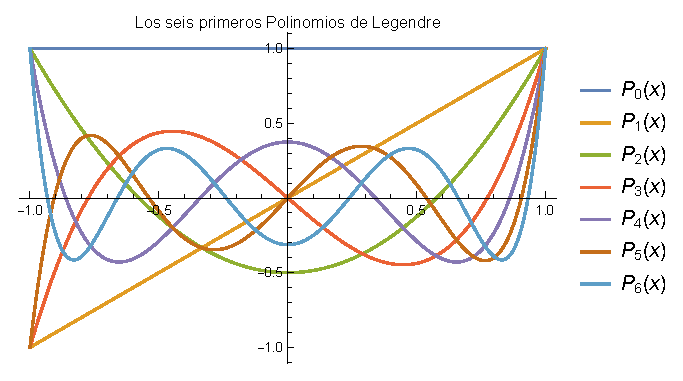
\includegraphics[scale=0.95]{Imagenes/Plot_Lagrange_0-6.eps}
\end{figure}
\end{frame}
\begin{frame}
\frametitle{Revisando los $P_{l}(x)$}
La gráfica de los  sugiere que los máximos y mínimos relativos de los $P_{n} (x)$ disminuyen de tamaño al aumentar $n$.
\\
\bigskip
\pause
Esto nos hace sospechar que el valor de la integral de $[P_{n} (x)]^{2}$ disminuirá a medida que $n$ aumente, quizás hacia el límite cero cuando $n  \to \infty$.
\end{frame}
\begin{frame}
\frametitle{Revisando los $P_{l}(x)$}
Pero estas observaciones no dan mucha pista sobre el valor real de la integral.
\\
\bigskip
\pause
Debemos buscar más si queremos deducir la fórmula deseada para el valor real de la integral.
\end{frame}
\begin{frame}
\frametitle{Propuesta de solución}
Tendríamos oportunidad de resolver el problema si de alguna manera podemos escribir el integrando $[P_{n} (x)]^{2}$ como un producto que involucra una derivada.
\end{frame}
\begin{frame}
\frametitle{Propuesta de solución}
Deberíamos de considerar entonces la fórmula de Rodrigues para los $P_{n} (x)$:
\pause
\begin{align*}
P_{n}(x) = \dfrac{1}{2^{n} \, n!} \dv[n]{x} (x^{2} - 1)^{n}
\end{align*}
\end{frame}
\begin{frame}
\frametitle{Propuesta de solución}
Que nos permite escribir:
\pause
\begin{eqnarray*}
\begin{aligned}
&\scaleint{6ex}_{\bs -1}^{1} \bigg[ P_{n}(x) \bigg]^{2} \dd{x} = \pause \scaleint{6ex}_{\bs -1}^{1} \bigg[ \dfrac{1}{2^{n} \, n!} \dv[n]{x} (x^{2} - 1)^{n} \bigg]^{2} \dd{x} = \\[0.5em] \pause
&= \dfrac{1}{2^{2n} \, (n!)^{2}} \, \scaleint{6ex}_{\bs -1}^{1} \bigg[ \dv[n]{x} (x^{2} - 1)^{n} \bigg] \, \bigg[ \dv[n]{x} (x^{2} - 1)^{n} \bigg] \dd{x}
\end{aligned}
\end{eqnarray*}
\end{frame}
\begin{frame}
\frametitle{Resolviendo la integral}
Ahora podemos aplicar la integración por partes a la integral del segundo renglón. \pause Esta integral, además de su coeficiente, es igual a:
\pause
\begin{eqnarray*}
\begin{aligned}
&\bigg[ \dv[n]{x} (x^{2} - 1)^{n} \cdot \dv[n-1]{x} (x^{2} - 1)^{n} \bigg] \Bigg\lvert_{-1}^{1} + \\[0.5em] \pause
&- \scaleint{6ex}_{\bs -1}^{1} \bigg[ \dv[n-1]{x} (x^{2} - 1)^{n} \bigg] \, \bigg[ \dv[n+1]{x} (x^{2} - 1)^{n} \bigg] \dd{x}
\end{aligned}
\end{eqnarray*}
\end{frame}
\begin{frame}
\frametitle{Valor de una parte de la integral}
La parte del integrando en los corchetes:
\pause
\begin{align*}
\bigg[ \dv[n]{x} (x^{2} - 1)^{n} \cdot \dv[n-1]{x} (x^{2} - 1)^{n} \bigg] \Bigg\lvert_{-1}^{1}
\end{align*}
se anula, \pause ya que la derivada de orden $(n - 1)$ de $(x^{2} - 1)^{n}$ contiene el factor $x^{2} - 1$, \pause por lo tanto se anula en $x = 1$ y $x = -1$.
\end{frame}
\begin{frame}
\frametitle{Avanzando en la solución}
Aplicando la integración por partes en la integral que nos queda, nos lleva a:
\begin{eqnarray*}
\begin{aligned}
&- \bigg[ \dv[n+1]{x} (x^{2} - 1)^{n} \cdot \dv[n-2]{x} (x^{2} - 1)^{n} \bigg] \Bigg\lvert_{-1}^{1} + \\[0.5em] \pause
&+ (-1)^{2} \scaleint{6ex}_{\bs -1}^{1} \bigg[ \dv[n-2]{x} (x^{2} - 1)^{n} \bigg] \, \bigg[ \dv[n+2]{x} (x^{2} - 1)^{n} \bigg] \dd{x}
\end{aligned}
\end{eqnarray*}    
\end{frame}
\begin{frame}
\frametitle{Avanzando en la solución}
La parte del integrando en corchetes nuevamente se anula. \pause Si repetimos el procedimiento $n$ veces, llegamos a:
\pause
\begin{align*}
\scaleint{6ex}_{\bs -1}^{1} \bigg[ P_{n}(x) \bigg]^{2} \dd{x} &= \dfrac{(-1)^{n}}{2^{2n} (n!)^{2}} \times \\[0.5em]
&\times \scaleint{6ex}_{\bs -1}^{1} \big ( x^{2} {-} 1 \big) \dv[2n]{x} (x^{2} {-} 1)^{n} \dd{x}
\end{align*}
\end{frame}
\begin{frame}
\frametitle{Revisando el integrando}
Al revisar el segundo factor del integrando, vemos que:
\begin{eqnarray*}
&{}&\displaystyle \dv[2n]{x} (x^{2} - 1)^{n} = \\[0.5em] \pause
&=& \displaystyle \dv[2n]{x} \big[ x^{2n} + c_{1} x^{2n-2} + c_{2} x^{2n-4} + \cdots + c_{2n} \big]
\end{eqnarray*}
\pause
donde $c_{1}, c_{2}, \ldots, c_{n}$ son coeficientes constantes.
\end{frame}
\begin{frame}
\frametitle{La derivada de orden $2n$}
Para cuando diferenciamos el polinomio entre corchetes $2n$ veces, la segunda derivada de cada término se habrá convertido en cero, \pause excepto la del primer término, cuya segunda derivada es $(2 \, n)!$.
\end{frame}
\begin{frame}
\frametitle{Resultado parcial}
Por lo tanto, la integral inicial se convierte en:
\pause
\begin{align*}
\scaleint{6ex}_{\bs -1}^{1} \bigg[ P_{n}(x) \bigg]^{2} \dd{x} = \pause \dfrac{(-1)^{n} \, (2n)!}{2^{2n} (n!)^{2}} \, \scaleint{6ex}_{\bs -1}^{1} (x^{2} - 1)^{n} \dd{x}
\end{align*}
\\
\bigskip
\pause
Como:
\begin{align*}
(-1)^{n} \, (x^{2} - 1)^{n} = (1 - x^{2})^{n}
\end{align*}
\end{frame}
\begin{frame}
\frametitle{Completando la expresión}
Si colocamos $x^{0}$ en el integrando, se tiene que: \pause
\begin{eqnarray*}
\scaleint{6ex}_{\bs -1}^{1} \bigg[ P_{n}(x) \bigg]^{2} \dd{x} = \pause \dfrac{(2 \, n)!}{2^{2n} (n!)^{2}} \, 2 \, \scaleint{6ex}_{\bs 0}^{1} x^{0} \, (1 - x^{2})^{n} \dd{x}
\end{eqnarray*}

\pause
De donde reconocemos que es una integral Beta, con $a = 1$, $b = 0$, $c = 2$ y $d = n$. Al ocupar la correspondiente expresión para esta integral, veremos que:
\end{frame}
\begin{frame}
\frametitle{Resultado de la integral}
Se tiene entonces que:
\pause
\begin{align*}
\scaleint{6ex}_{\bs -1}^{1} \bigg[ P_{n}(x) \bigg]^{2} \dd{x} = \pause \dfrac{2 \, (2 \, n)!}{2^{2n} \, (n!)^{2}} \, \dfrac{\Gamma(1/2) \, \Gamma(n + 1)}{(2 n + 1) \, \Gamma (n + [1/2])}
\end{align*}
\end{frame}
\begin{frame}
\frametitle{Usando una expresión}
Para $(2 n)!$ escribimos $2 \, n \, \Gamma (2n)$, y de la fórmula de duplicación de Legendre, tenemos que:
\begin{align*}
\Gamma( 2 \, n) = \dfrac{\Gamma (n) \, \Gamma [n + (1/2)]}{2^{1-2n} \, \Gamma(1/2)}
\end{align*}
\end{frame}
\begin{frame}
\frametitle{Conclusión}
Sustituyendo este valor de $\Gamma(2n)$, llegamos a:
\pause
\begin{eqnarray*}
\scaleint{6ex}_{\bs -1}^{1} \bigg[ P_{n}(x) \bigg]^{2} \dd{x} = \pause \dfrac{2}{2 \, n + 1} \qed
\end{eqnarray*}
\end{frame}

%Ref. Farrell IV-9
\section{Ejercicio con una esfera}
\frame{\tableofcontents[currentsection, hideothersubsections]}
\subsection{Planteamiento}

\begin{frame}
\frametitle{Enunciado del ejercicio}
Determina la distribución de temperatura $T$ en estado estacionario en una esfera sólida cuando un hemisferio (excluyendo una franja de separación) se mantiene a $\SI{300}{\degreeCelsius}$, \pause mientras que el otro hemisferio (excluyendo la franja de separación) se mantiene a $\SI{75}{\degreeCelsius}$, \pause la temperatura de la franja puede considerarse indefinida.
\end{frame}
\begin{frame}
\frametitle{Representación gráfica}
\begin{figure}
    \centering
    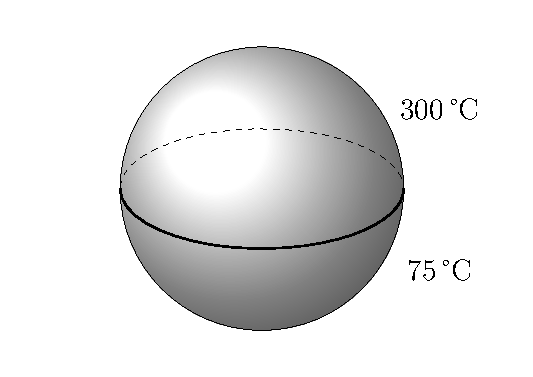
\includegraphics[scale=1.2]{Imagenes/esfera_Clase_19.eps}
\end{figure}
\end{frame}
\begin{frame}
\frametitle{Ecuación de calor}
La solución para la ecuación para la conducción de calor en un sólido es:
\pause
\begin{align}
\pdv{T}{t} = \dfrac{k}{\rho \, c} \big( \laplacian{T} + \pderivada{Q} \big)
\label{eq:ecuacion_9_01}
\end{align}
donde $T$ es la temperatura, $t$ el tiempo, $k$ es la conductividad térmica, $\rho$ es la densidad, $c$ es el calor específico y $\pderivada{Q}$ es la razón para el calor generado.
\end{frame}
\begin{frame}
\frametitle{Condición en el ejercicio}
En el ejercicio $\pderivada{Q} = 0$ ya que no hay calor generado, \pause $T$ es independiente del tiempo por lo que $\pdv*{T}{t} = 0$.
\\
\bigskip
\pause
Tomemos la esfera sólida con centro en el origen y con el sistema de coordenadas esféricas $(r, \theta, \phi)$, donde $r$ es la distancia del origen, $\phi$ es el ángulo de colatitud o polar, y $\theta$ es el ángulo azimutal.
\end{frame}
\begin{frame}
\frametitle{Orientación de los hemisferios}
Sea el sistema de coordenadas orientado de modo que la superficie del hemisferio $0 \leq \phi < \pi/2$, es la que está a $\SI{300}{\degreeCelsius}$.
\\
\bigskip
\pause
Luego por simetría de la temperatura en la superficie, se deduce que la distribución de temperatura $T$ dentro del sólido y la superficie es independiente de $\theta$.
\end{frame}

\subsection{Ecuación de calor}

\begin{frame}
\frametitle{Ecuación de calor para el ejercicio}
Por lo que para el ejercicio se tiene que:
\pause
\begin{align}
\laplacian{T} = 0
\label{eq:ecuacion_9_02}
\end{align}
con $T = T(r, \phi)$, de este modo la ecuación de Laplace escrita en términos de coordenadas esféricas, donde $T$ no depende de $\theta$ es:
\pause
\begin{align}
\pdv{r} \left( r^{2} \pdv{T}{r} \right) + \dfrac{1}{\sin \phi} \pdv{\phi} \left( \sin \phi \pdv{T}{\phi} \right) = 0
\label{eq:ecuacion_9_03}
\end{align}
\end{frame}
\begin{frame}
\frametitle{¿Qué debemos de resolver?}
Entonces nuestro problema es encontrar $T$ como una función de $r$ y $\phi$ que satisface la ecuación (\ref{eq:ecuacion_9_03}) dentro de la esfera sólida y tomando los valores límites de temperatura preescritos en la superficie.
\end{frame}

\subsection{Separación de variables}

\begin{frame}
\frametitle{Separando la ecuación}
Ocupamos la técnica de separación de variables, tal que:
\pause
\begin{align}
T = F \, G = f(r) \, g(\phi)
\label{eq:ecuacion_9_04}
\end{align}
\end{frame}
\begin{frame}
\frametitle{Haciendo la separación}
Por lo que al tomar la primera y segunda derivada de $T$ con respecto a $r$ y $\phi$, se tiene:
\pause
\begin{align}
\pdv{T}{r} &= \pderivada{F} \, G \hspace{0.2cm} \Rightarrow \hspace{0.2cm} \pdv[2]{T}{r} = \sderivada{F} \, G \label{eq:ecuacion_9_05} \\[0.5em]
\pdv{T}{\phi} &= F \, \pderivada{G} \hspace{0.2cm} \Rightarrow \hspace{0.2cm} \pdv[2]{T}{\phi} = F \, \sderivada{G} \label{eq:ecuacion_9_06} 
\end{align}
\end{frame}
\begin{frame}
\frametitle{Sustituyendo las derivadas}
Que al sustituir en la ec. (\ref{eq:ecuacion_9_03}), obtenemos:
\pause
\begin{align}
2 r \pderivada{F} G + r^{2} \sderivada{F} G + F \pderivada{G} \cot \phi + F \sderivada{G} = 0
\label{eq:ecuacion_9_07}
\end{align}
\end{frame}
\begin{frame}
\frametitle{Acomodando los términos}
Al reacomodar los términos de la ecuación:
\pause
\begin{align}
\dfrac{2 r \pderivada{F} + r^{2} \sderivada{F}}{F} = - \dfrac{\pderivada{G} \cot \phi + \sderivada{G}}{G}
\label{eq:ecuacion_9_08}
\end{align}
\end{frame}
\begin{frame}
\frametitle{La constante de separación}
Sea $C$ la constante de separación, de esta manera:
\pause
\begin{align}
\pderivada{G} \cot \phi + \sderivada{G} = - C \, G
\label{eq:ecuacion_9_09}
\end{align}
\end{frame}
\begin{frame}
\frametitle{Analizando la situación}
Consideremos el cambio en $T$ a medida que nos movemos hacia abajo en la mitad superior de la esfera a lo largo de una curva en la cual $r$ permanece constante.
\end{frame}
\begin{frame}
\frametitle{Analizando la situación}
Entonces el cambio en $T$ a lo largo de dicha curva se debe completamente al cambio en $G$. 
\\
\bigskip
\pause
Ahora bien, $T$ es ciertamente positivo en todo momento, si asumimos que $F$ y $G$ son ambas positivas, entonces $G$ disminuye a medida que avanzamos debajo a lo largo de la curva.
\end{frame}
\begin{frame}
\frametitle{Aplicando el razonamiento}
Este razonamiento mantiene la igualdad de la ec. (\ref{eq:ecuacion_9_04}) por lo tanto, la derivada $\pderivada{G}$ es negativa.
\\
\bigskip
\pause
En la mitad superior $\cot \phi$ es positivo.
\end{frame}
\begin{frame}
\frametitle{Aplicando el razonamiento}
Por lo que sería razonable considerar que la segunda derivada $\sderivada{G}$ sería negativa en la mitad superior, \pause lo que nos dice que la primera derivada negativa se está volviendo más negativa.
\\
\bigskip
\pause
El lado izquierdo de la ec. (\ref{eq:ecuacion_9_09}) sería negativo en la mitad superior. \pause Concluimos que $C$ debe ser positivo, \pause hagamos que $C = k^{2}, \, k \neq 0$.
\end{frame}
\begin{frame}
\frametitle{Las soluciones $F$ y $G$}
Ahora veamos si podemos encontrar soluciones para la ec. (\ref{eq:ecuacion_9_02}) de la forma $T = F \, G = f(r) \, g(\phi)$ donde $F$ y $G$ son ambas positivas tales que:
\pause
\begin{align}
\dfrac{2 r \pderivada{F} + r^{2} \sderivada{F}}{F} = - \dfrac{\pderivada{G} \cot \phi + \sderivada{G}}{G} = k^{2} \hspace{0.5cm} k \neq 0
\label{eq:ecuacion_9_10}
\end{align}
\end{frame}

\subsection{Sistema de dos EDO}

\begin{frame}
\frametitle{Sistema de dos EDO}
Entonces tendremos:
\begin{align}
r^{2} \, \sderivada{F} + 2 \, r \, \pderivada{F} - k^{2} \, F &= 0 \label{eq:ecuacion_9_11} \\[0.5em]
\sderivada{G} + \big[ \cot \phi \big] \, \pderivada{G} + k^{2} \, G &= 0 \label{eq:ecuacion_9_12}
\end{align}
\end{frame}
\begin{frame}
\frametitle{Solución para $G$}
Si hacemos $k^{2} = n(n + 1)$ la ec. (\ref{eq:ecuacion_9_12}) es una ecuación de Legendre con $G$ como $y$.
\\
\bigskip
\pause
La solución particular de (\ref{eq:ecuacion_9_12}) es:
\pause
\begin{align*}
G = C_{n} \, P_{n}(\cos \phi)
\end{align*}
con $C_{n}$ una constante arbitraria.
\end{frame}
\begin{frame}
\frametitle{Solución para F}
Con $k^{2} = n(n + 1)$ la solución general de la ec. (\ref{eq:ecuacion_9_11}) es:
\pause
\begin{align}
F = S_{n} \, r^{n} + \dfrac{B_{n}}{r^{n+1}}
\label{eq:ecuacion_9_13}
\end{align}
donde $S_{m}$ y $B_{n}$ son constantes arbitrarias.
\end{frame}
\begin{frame}
\frametitle{Evitando una singularidad}
El segundo término de la derecha en la ec. (\ref{eq:ecuacion_9_13}) \emph{tiende infinito} en $r = 0$ y esto no debe de suceder.
\\
\bigskip
\pause
Para evitar esto, hacemos que $B_{n} = 0$.
\end{frame}

\subsection{Solución general del problema}

\begin{frame}
\frametitle{Solución general del problema}
Entonces el producto de soluciones para la ec. (\ref{eq:ecuacion_9_02}) es de la forma:
\pause
\begin{align}
T = F \, G = S_{n} \, C_{n} \, r^{n} \, P_{n} (\cos \phi)
\label{eq:ecuacion_9_14}
\end{align}
pero ninguna solución en particular cumplirá las CDF:
\begin{align}
T(R, \phi) = \begin{cases}
\SI{300}{\degreeCelsius} & 0 \leq \phi < \dfrac{\pi}{2} \\
\SI{75}{\degreeCelsius} & \dfrac{\pi}{2} < \phi \leq \pi \\
\end{cases}
\label{eq:ecuacion_9_15}
\end{align}
\end{frame}
\begin{frame}
\frametitle{Los $P_{n}(\cos \phi)$ son funciones continuas}
Para hacerlo sería necesario que $P_{n} (\cos \theta)$ \emph{mantenga un valor constante} para $0 \leq \phi < \pi/2$ \pause y \emph{mantenga otro valor constante} para $\pi/2 < \phi \leq \pi$.
\\
\bigskip
\pause
!Esto no es posible¡ \pause Los polinomios ordinarios de Legendre \textbf{son funciones continuas del argumento}.
\end{frame}

\subsection{La continuidad de los \texorpdfstring{$P_{n}(\cos \theta)$}{Pn(cos t)}}

\begin{frame}
\frametitle{Forma de resolver la continuidad}
Sin embargo, podemos cumplir las CDF de la siguiente manera: \pause sea $T_{E}$ el exceso de temperatura  $T$ en la mitad superior de la superficie sobre la de $T$ en la mitad inferior.
\\
\bigskip
\pause
En la franja de separación, definimos de manera arbitraria $T_{E} = \dfrac{\SI{225}{\degreeCelsius}}{2}$.
\end{frame}
\begin{frame}
\frametitle{Ajustando las CDF}
Así:
\begin{align}
T_{E} = \begin{cases}
\SI{225}{\degreeCelsius} & 0 \leq \phi < \dfrac{\pi}{2} \\
0 & \dfrac{\pi}{2} < \phi \leq \pi \\
\dfrac{\SI{225}{\degreeCelsius}}{2} & \phi = \dfrac{\pi}{2}
\end{cases}
\label{eq:ecuacion_9_16}
\end{align}
\end{frame}
\begin{frame}
\frametitle{Cambiando de variable}
Si hacemos que $x = \cos \phi$, entonces $T_{E}(\phi)$ será $f(x)$, y queda definida como:
\begin{align}
f(x) = \begin{cases}
\SI{225}{\degreeCelsius} & 0 < x \leq 1 \\
0 & -1 \leq x < 0 \\
\dfrac{\SI{225}{\degreeCelsius}}{2} & x = 0
\end{cases}
\label{eq:ecuacion_9_17}
\end{align}
\end{frame}

\subsection{Expandiendo una función}

\begin{frame}
\frametitle{Expandiendo la función $f(x)$}
Ahora podemos expandir la función $f(x)$ en términos de los polinomios ordinarios de Legendre:
\pause
\begin{align*}
f(x) = \nsum_{n=0}^{\infty} A_{n} \, P_{n} (x)
\end{align*}
donde:
\pause
\begin{align*}
A_{n} = \dfrac{2 \, n + 1}{2} \scaleint{6ex}_{0}^{1} f(x) \, P_{n}(x) \dd{x}
\end{align*}
\end{frame}
\begin{frame}
\frametitle{Resultado de la expansión}
Entonces la función $f(x)$ resulta ser:
\pause
\begin{align}
f(x) &= \SI{225}{\degreeCelsius} \bigg[ \dfrac{1}{2} {+} \dfrac{3}{4} P_{1}(x) {-} \dfrac{7}{16} P_{3}(x) + \\[0.5em]
&+ \dfrac{11}{32} P_{5} (x) - \cdots \bigg]
\label{eq:ecuacion_9_18}
\end{align}
\end{frame}
\begin{frame}
\frametitle{Regresando a la solución}
Volviendo a la ec. (\ref{eq:ecuacion_9_14}), elegimos las constantes $S_{n} \, C_{n}$ con $n = 0,1 ,2, \ldots$ de modo que para cada $n$, tomamos:
\pause
\begin{align}
S_{n} \, C_{n} = \dfrac{A_{n}}{R^{n}}
\end{align}
donde $A_{n}$ es el coeficiente de $P_{n}(x)$ de la ec. (\ref{eq:ecuacion_9_18}) y $R$ es el radio de la esfera.
\end{frame}

\subsection{Solución completa}

\begin{frame}
\frametitle{Solución completa}
Componiendo una serie infinita de tan particular soluciones, tomamos:
\begin{eqnarray}
\begin{aligned}[t]
&T(r, \phi) = \SI{75}{\degreeCelsius} {+} \nsum_{n=0}^{\infty} A_{n} \, \bigg( \dfrac{r}{R} \bigg)^{n} \, P_{n} (\cos \phi) = \\[0.5em] \pause
&= \SI{75}{\degreeCelsius} + \SI{225}{\degreeCelsius} \bigg[ \dfrac{1}{2} {+} \dfrac{3}{4} \bigg( \dfrac{r}{R} \bigg) P_{1} (\cos \phi)  + \\[0.5em]
&- \dfrac{7}{16} \bigg( \dfrac{r}{R} \bigg)^{3} P_{3} (\cos \phi) {+} \dfrac{11}{32} \bigg( \dfrac{r}{R} \bigg)^{5} P_{5} (\cos \phi) - \ldots  \bigg]
\end{aligned}
\label{eq:ecuacion_9_21}
\end{eqnarray}
\end{frame}
\begin{frame}
\frametitle{Revisando la convergencia de la solución}
El lado derecho de la ecuación converge por la ec. (\ref{eq:ecuacion_9_18}) a la distribución de temperatura superficial prescrita cuando $r = R$
\\
\bigskip
\pause
Este lado derecho también será convergente para $r < R$ en virtud del factor $\left( \dfrac{r}{R} \right)^{n}$.
\end{frame}
\begin{frame}
\frametitle{Conclusión}
Cada término de la derecha satisface individualmente la ecuación de Laplace y la convergencia es tal que la serie de Laplacianos de los términos individuales convergen a cero para $r < R$.
\\
\bigskip
Por lo tanto, la ec. (\ref{eq:ecuacion_9_21}) proporciona la solución a nuestro problema.
\end{frame}
\begin{frame}
\frametitle{Observación final}
Como se señaló anteriormente, la función de temperatura $T$ hace lo mejor que podría esperarse de ella en la franja que separa las mitades de la superficie limítrofe, ya que asume allí el promedio de las dos temperaturas constantes diferentes.
\end{frame}

\end{document}